\chapter{The Special Environments\\Quotation and Quote}

\begin{quotation}
\lipsum[1-2]
\end{quotation}

\begin{figure}
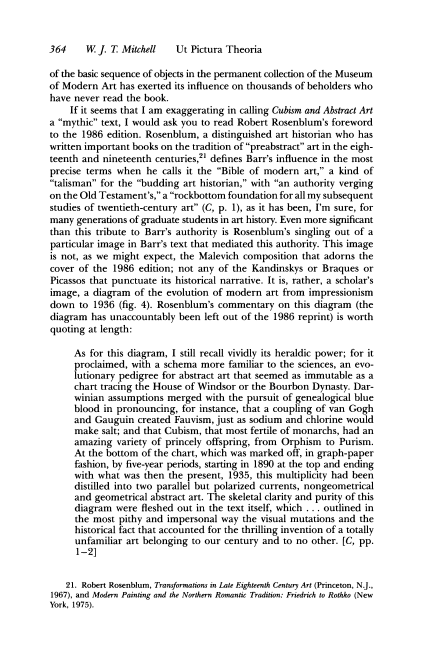
\includegraphics[width=0.9\linewidth]{quotations-01}
\caption{Most books have quotes flushed right.}
\end{figure}

%% Set the quotation environment
\cxset{
  quotation above/.store in=\quotationabove@cx,
  quotation left margin/.store in=\quotationleftmargin@cx,
  quotation right margin/.store in=\quotationrightmargin@cx,
  quotation parsep/.store in=\quotationparsep@cx,
  quotation font-size/.store in=\quotationfontsize@cx,
  quotation parindent/.store in=\quotationparindent@cx,
}

\def\setquotation#1{%
\cxset{#1}
\renewenvironment{quotation}
               {\par\addvspace{\quotationabove@cx}
                \list{}{\listparindent\quotationparindent@cx%
                        \leftmargin=\quotationleftmargin@cx%
                        \itemindent    \listparindent
                        \rightmargin   \leftmargin
                        \parsep=\quotationparsep@cx%
                        \quotationfontsize@cx}%
                \item\relax\hskip-\listparindent}
               {\endlist}
}

% Some default values
\setquotation{%
  quotation above=6pt,
  quotation left margin=20pt,
  quotation right margin=0pt,
  quotation parsep=0pt,
  quotation font-size=\small,
  quotation parindent=12pt,
}

%% Set the quote environment
\cxset{
  quote above/.store in=\quoteabove@cx,
  quote left margin/.store in=\quoteleftmargin@cx,
  quote right margin/.store in=\quoterightmargin@cx,
  quote parsep/.store in=\quoteparsep@cx,
  quote font-size/.store in=\quotefontsize@cx,
  quote parindent/.store in=\quoteparindent@cx,
}

\def\setquote#1{%
\cxset{#1}
\renewenvironment{quote}
               {\par\addvspace{\quoteabove@cx}
                \list{}{\listparindent\quoteparindent@cx%
                        \leftmargin=\quoteleftmargin@cx%
                        \itemindent    \listparindent
                        \rightmargin   \leftmargin
                        \parsep=\quoteparsep@cx%
                        \quotefontsize@cx}%
                \item\relax\hskip-\listparindent}
               {\endlist}
}

% Some default values
\setquotation{%
  quotation above=36pt,
  quotation left margin=50pt,
  quotation parsep=0pt,
  quotation font-size=\small,
  quotation parindent=12pt,
}
\setquote{%
  quote above=36pt,
  quote left margin=20pt,
  quote parsep=0pt,
  quote font-size=\small,
  quote parindent=12pt,
}

\section{Quotation}
In the standard \LaTeXe\ classes the quotation and quote environment are defined by making clever use of the list environment. The main difference between the quotation and the quote environment is that the first line of the former is indented. The key value interface for the quotation environment is shown below and a similar one exists for the quotation environment:

\section{Key-value interface}\index{quotation!keys}

\keyval{quote above}{\marg{dim}}{Skip dimension for above quotation skip.}
\keyval{quote below}{\marg{dim}}{Skip dimension for below quotation skip.}
\keyval{quote parindent}{\marg{dim}}{Paragraph indentation.}
\keyval{quote parsep}{\marg{dim}}{Paragraph below skip.}
\keyval{quote left margin}{\marg{dim}}{Paragraph below skip.}
\keyval{quote right margin}{\marg{dim}}{Paragraph below skip.}

\index{quotation!example}
\begin{tcblisting}{title=Quotation environment example,width=\textwidth}
\setquotation{%
  quotation above=36pt,
  quotation left margin=0pt,
  quotation right margin=0pt,
  quotation parsep=10pt,
  quotation font-size=\small,
  quotation parindent=1em,
}
\begin{quotation}
\lipsum[2-3]
\end{quotation}
\end{tcblisting}

\section{Quote}
This is the quote environment:
\begin{quote}
\lipsum[1-2]
\end{quote}
